\documentclass[xcolor=x11names,compress]{beamer}
\usepackage[english]{babel}

%% General document %%%%%%%%%%%%%%%%%%%%%%%%%%%%%%%%%%
\usepackage{graphicx}
\usepackage{tikz}
\usepackage{wrapfig}
\usepackage{hyperref}

\usetikzlibrary{decorations.fractals}
%%%%%%%%%%%%%%%%%%%%%%%%%%%%%%%%%%%%%%%%%%%%%%%%%%%%%%


%% Beamer Layout %%%%%%%%%%%%%%%%%%%%%%%%%%%%%%%%%%
\useoutertheme[subsection=false,shadow]{miniframes}
\useinnertheme{default}
\usefonttheme{serif}
\usepackage{palatino}

\setbeamerfont{title like}{shape=\scshape}
\setbeamerfont{frametitle}{shape=\scshape}

\setbeamercolor*{lower separation line head}{bg=DeepSkyBlue4} 
\setbeamercolor*{normal text}{fg=black,bg=white} 
\setbeamercolor*{alerted text}{fg=red} 
\setbeamercolor*{example text}{fg=black} 
\setbeamercolor*{structure}{fg=black} 
 
\setbeamercolor*{palette tertiary}{fg=black,bg=black!10} 
\setbeamercolor*{palette quaternary}{fg=black,bg=black!10} 

\renewcommand{\(}{\begin{columns}}
\renewcommand{\)}{\end{columns}}
\newcommand{\<}[1]{\begin{column}{#1}}
\renewcommand{\>}{\end{column}}
%%%%%%%%%%%%%%%%%%%%%%%%%%%%%%%%%%%%%%%%%%%%%%%%%%
\newcommand{\hlb}[1]{\textbf{\textcolor{blue}{#1}}}
\newcommand{\hl}[1]{\textcolor{blue}{#1}}
\newcommand{\lien}[2]{\mathcal{L}_{#1}^{#2}}
\newcommand{\lie}[1]{\mathcal{L}_{#1}}

%\usepackage[english]{babel}
\usepackage[utf8]{inputenc}
%\usetheme{Goettingen}

\begin{document}
\title{Bifurcations in continuous time dynamical systems}
\author{Debsankha Manik}

\begin{frame}

%opening

\titlepage

\end{frame}
\section{Monodromy matrix}
\begin{frame}{Poincare section for non-autonomous systems}
\[
t\mod{T}=0
\]
\begin{figure}
\begin{center}
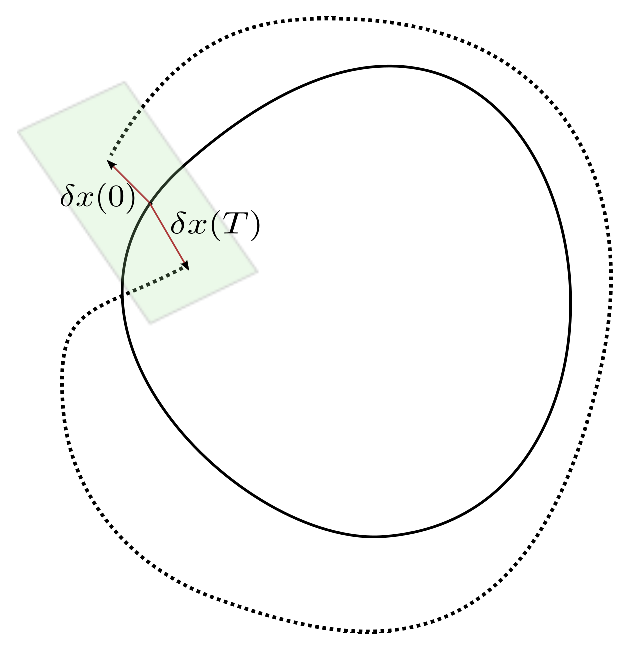
\includegraphics[width=0.28\columnwidth]{monodromy}
\end{center}
\end{figure}

The Poincare map:
\[
x(T)=f(T)x(0)
\]


The Poincare map can be locally linearized in the neighbourhood of a fixed point:
\[
\delta x(T)=M(T)\delta x(0)
\]
\end{frame}

\begin{frame}{The Monodromy Matrix}
\[
\delta x(T)=M(T)\delta x(0)
\]

The eigenvalues of $M$ determine the stability of the fixed point.   
\begin{figure}
\begin{center}
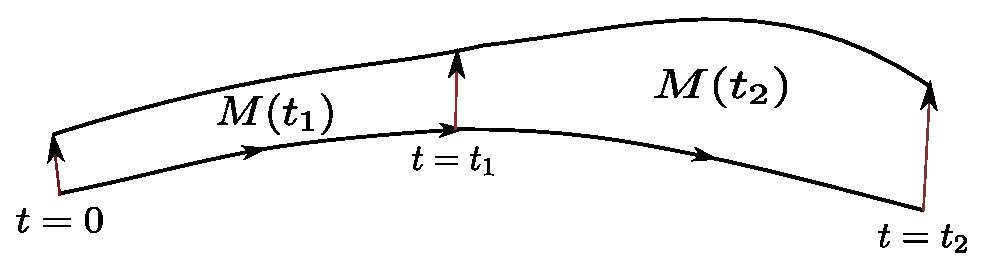
\includegraphics[width=0.9\columnwidth]{multiplicity}
\end{center}
\end{figure}


$\delta x(t_1+t_2)=M(t_2)M(t_1)\delta x(0)=M(t_1+t_2)\delta x(0)$
Clearly, $M(t_1+t_2)=M(t_1+t_2)$.  

\end{frame}

\section{Saltation matrix}
\begin{frame}{What about border collision?}
\begin{figure}
\begin{center}
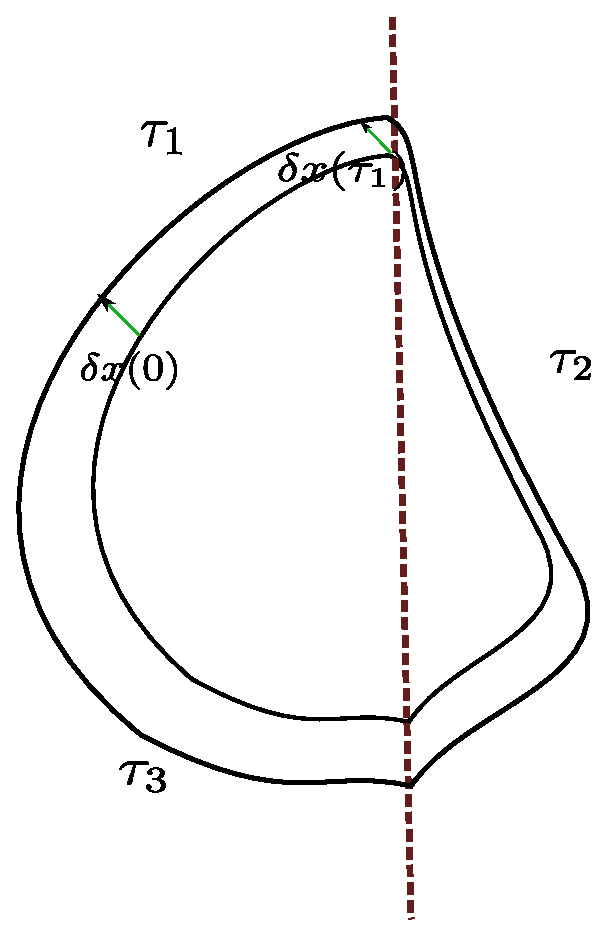
\includegraphics[width=0.3\columnwidth]{border-c}
\end{center}
\end{figure}

\[
M\neq M(\tau_3)M(\tau_2)M(\tau_1)
\]

Although $x$ and $x+\delta x$ start close by, they do not hit the boundary 
simultaneously. So some correction factor must be applied to $M$.  

\end{frame}

\begin{frame}{Saltation matrix}
\begin{figure}
\begin{center}
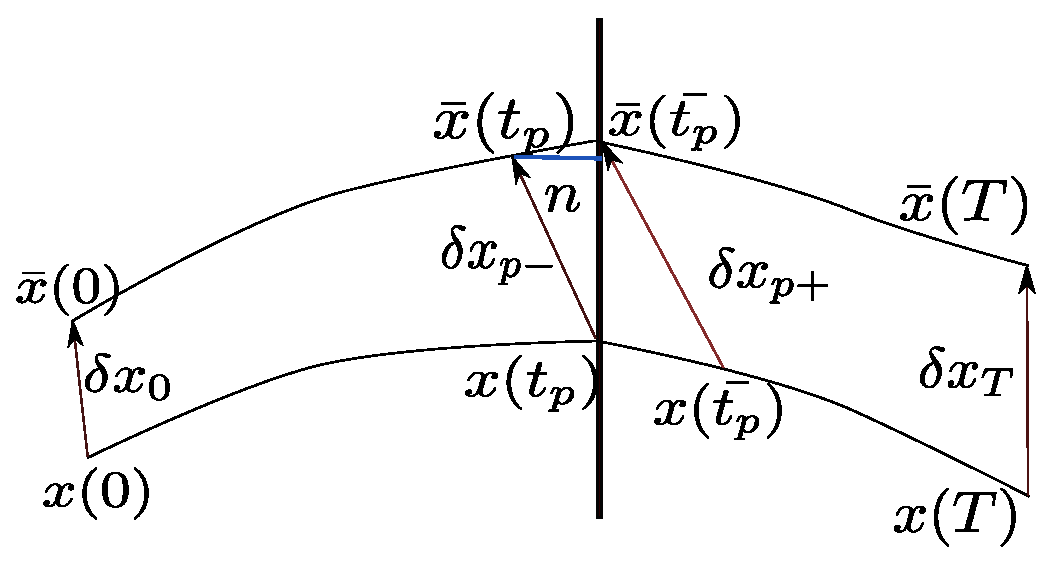
\includegraphics[width=0.6\columnwidth]{saltation}
\end{center}
\end{figure}

We know that $M(T)\neq M(T-t_p)M(t_p)$.  What is the correction factor?\\
\pause{}

We need to find out $S$ satisfying:
\[
\delta x_{p+}=S\delta  x(p-)
\]

Let $\delta t=\bar{t_p}-t_p$\\
\end{frame}

\begin{frame}
\begin{figure}
\begin{center}
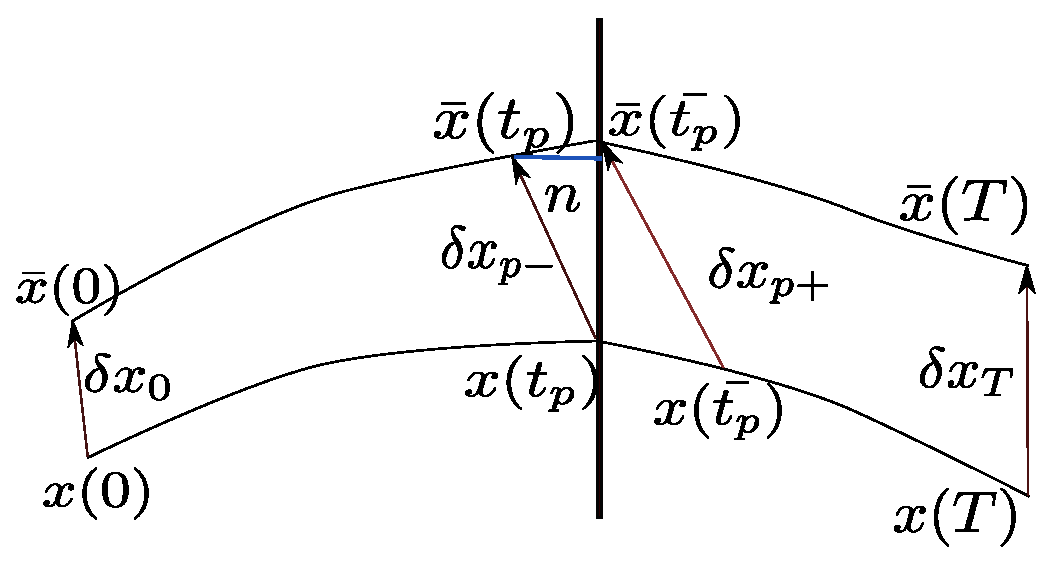
\includegraphics[width=0.6\columnwidth]{saltation}
\end{center}
\end{figure}

\begin{equation}
\label{eq-salt-barx}
\bar{x}(\bar{t_p})=\bar{x}(t_p)+f_{p-}\delta t
\end{equation}

\begin{equation}
\label{eq-salt-x}
x(\bar{t_p})=x(t_p)+f_{p+}\delta t
\end{equation}

Subtracting:
\begin{equation}
\delta x_{p+}=\delta x_{p-}+(f_{p-}-f_{p+})\delta t
\end{equation}
\end{frame}

\begin{frame}
\begin{figure}
\begin{center}
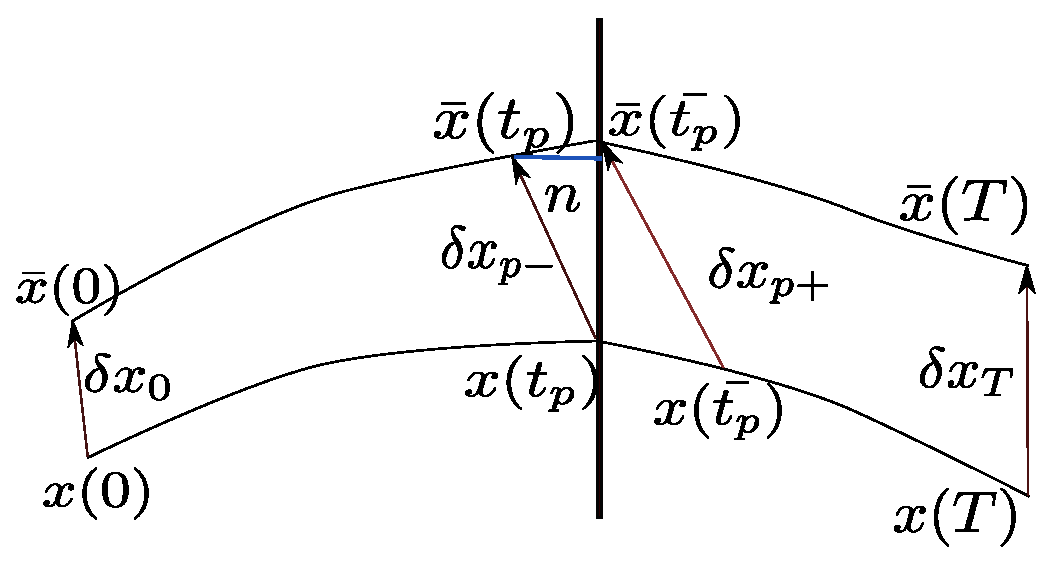
\includegraphics[width=0.6\columnwidth]{saltation}
\end{center}
\end{figure}

To evaluate $\delta t$, note that:
\begin{eqnarray}
n^Tf_{p-}\delta t&=&-n^T\delta x_{p-}\\
\delta t&=&-\frac{n^T\delta x_{p-}}{n^Tf_{p-}} \\
\delta x_{p+}&=&\delta x_{p-}+(f_{p+}-f_{p-})\frac{n^T\delta x_{p-}}{n^Tf_{p-}}\\
S&=&I+\frac{(f_{p+}-f_{p-})n^T}{n^Tf_{p-}}
\end{eqnarray}

\end{frame}

\section{Poincare map after border collision}
\begin{frame}
\begin{figure}
\begin{center}
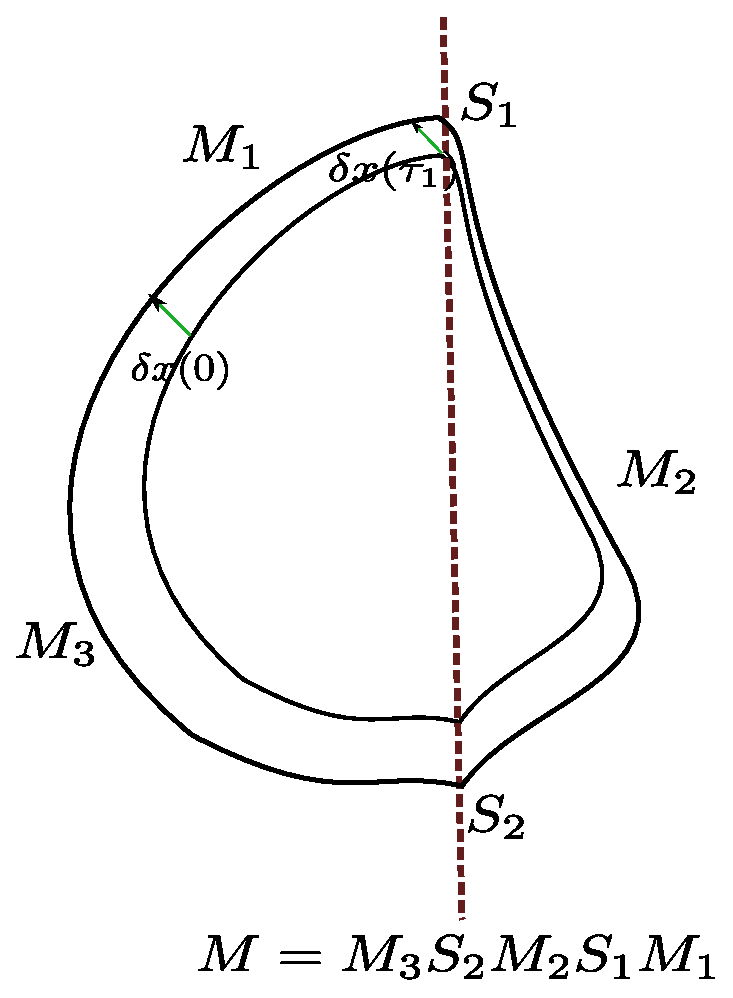
\includegraphics[width=0.4\columnwidth]{border-c-salt}
\end{center}
\end{figure}

\end{frame}

\begin{frame}{Soft impact in simple harmonic oscillator}
\begin{figure}
\caption{}
\begin{center}
\includegraphics[width=0.6\columnwidth]{osc-pw}
\end{center}
\end{figure}

\hlb{The non-forced case:}

\begin{eqnarray}
X&=&\begin{bmatrix}
x\\v
\end{bmatrix}\\
F_1(X)&=&\begin{bmatrix}
0 & 1\\
-k_1 & 0
\end{bmatrix}
\begin{bmatrix}
x\\v
\end{bmatrix}
\end{eqnarray}
\end{frame}

\begin{frame}
\begin{eqnarray}
F_2(X)&=&\begin{bmatrix}
0 & 1\\
-k_1-k_2 & 0
\end{bmatrix}
\begin{bmatrix}
x\\v
\end{bmatrix}
\end{eqnarray}

\begin{figure}
\caption{One trajectory}
\begin{center}
\includegraphics[width=0.6\columnwidth]{trajectory}
\end{center}
\end{figure}

\end{frame}


\begin{frame}{Monodromy Matrix}
\begin{eqnarray*}
X(t)&=&\exp{\left(
\begin{bmatrix}
0 & 1\\
-k_1 & 0
\end{bmatrix}t\right)}
\begin{bmatrix}
x(0)\\v(0)
\end{bmatrix}\\
&=&\begin{bmatrix}
\text {Cos}(t w) & \frac {\text {Sin}(t w)} {w}\\
-w\text {Sin}(t w) &  \text {Cos}(t w)
\end{bmatrix}
\begin{bmatrix}
x(0)\\v(0)
\end{bmatrix}
\end{eqnarray*}

($k=w^2$)\\

\begin{eqnarray}
S&=&I+\frac{(f_{p+}-f_{p-})n^T}{n^Tf_{p-}}\\
&=&I+
\begin{bmatrix}
0 & 0\\
-k_2x & 0 
\end{bmatrix}/v
\end{eqnarray}
\end{frame}


\begin{frame}{Monodromy Matrix}
\begin{figure}
\caption{Undamped case}
\begin{center}
\includegraphics[width=0.5\columnwidth]{nodamp}
\end{center}
\end{figure}

\[
M(T)= M(\tau_3)\cdot S_2\cdot M'(\tau_2)\cdot S_1\cdot M(\tau_1)
\]

Now, $det(M)=det(M')=1$\\
$det(S_1)=det(S_2)=1$ as well.  \\

Therefore all periodic orbits are neither attracting nor repelling
\end{frame}

\begin{frame}[label=BackFromSHMFormula]{Driven, damped Case}
\begin{eqnarray*}
F_1=-k_1x-G_1v+Fcos(\omega t)\\
F_2=-(k_1+k_2)x-G_1v+Fcos(\omega t)
\end{eqnarray*}


The full solution:\\
\[
x(t,x_0,v_0)=x_p(t)+x_h(t,x_0,v_0)
\]

\hyperlink{SHM-driven}{\beamergotobutton{Go to solution}}

Initial condition affects $x_h$ \emph{only}.\\
Therefore, $\delta X(t)$ is not dependent on the forcing function at all.  \\

Moreover:\[
X_h(t)=O\begin{bmatrix}e^{\lambda_+t} & 0\\0 & e^{\lambda_-t}\end{bmatrix}O^{-1}
\]

Where $\lambda_\pm=\frac{-G\pm\sqrt{G^2-4k}}{2}$\\
Therefore, $det(M)=exp(-G)$
\end{frame}

\begin{frame}
\begin{figure}
\begin{center}
\includegraphics[width=0.6\columnwidth]{withdamp}
\end{center}
\end{figure}

As before, 
\[
M(T)= M(\tau_3)\cdot S_2\cdot M'(\tau_2)\cdot S_1\cdot M(\tau_1)
\]

$det(M),det(M')<1$\\
$det(S_1)=det(S_2)=1$, as before.  \\

Therefore $det(M_{total})<1$

\end{frame}


\begin{frame}
But that implies there can be no chaos in this kind of systems.\\
\pause{}
It is not 
true:
\begin{figure}
\begin{center}
\includegraphics[width=0.9\columnwidth]{soft-impact.png}
\end{center}
\end{figure}
\end{frame}

\begin{frame}
\begin{figure}
\begin{center}
\includegraphics[width=0.9\columnwidth]{soft-impact-zoomed}
\end{center}
\end{figure}
\end{frame}


\begin{frame}[label=SHM-driven]
\begin{eqnarray*}
\ddot{x}+G\dot{x}+kx&=&Fcos(\omega t)\\
x_p(t)&=&\frac{F}{(k-\omega^2)^2+\omega^2G^2}cos(\omega t+tan^{-1}\frac{\omega G}{\omega^2-k})\\
x_h(t)&=&O\begin{bmatrix}e^{\lambda_+t} & 0\\0 & e^{\lambda_-t}\end{bmatrix}O^{-1}\\
O&=&\begin{bmatrix}1 & 1 \\ \lambda_+ & \lambda_-\end{bmatrix}\\
\lambda_\pm&=&\frac{-G\pm\sqrt{G^2-4k}}{2}
\end{eqnarray*}

\hyperlink{BackFromSHMFormula}{\beamergotobutton{Back}}
\end{frame}
\end{document}
